\section{Conception}\label{concept}

To reach the scope of this project defined in chapter \ref{scope} an overall system architecture must be designed. The system, seen in figure \ref{fig:fist_conc_system}, consists of three main parts: \textit{Frontend}, \textit{Backend and Database} and \textit{AS-Pair}. The Backend and the Database are connected over an \textit{Interface}.\\

\begin{figure}[H]
    \centering
    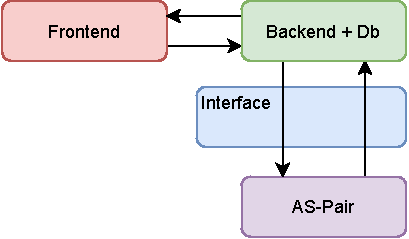
\includegraphics[width=.5\textwidth]{images/4_1/first_concept_ansicht.pdf}
    \caption{Schematic representation of the system}
    \label{fig:fist_conc_system}
\end{figure}

The \textit{Frontend} is the interface where interactions between humans and the rest of the system takes place. It is used to visualise the contents of the database and to control the communication with individual AS-Pairs.\\

The \textit{Backend} serves as a link between the frontend and the AS-Pairs. All interactions and information between the frontend, AS-Pairs and database are routed, controlled and logged via it. The work of the backend is supported by a \textit{database}. This stores information about the system which can be queried at a later time. The database could also be integrated externally.\\

The \textit{AS-Pairs} are the executing link of the system. They handle the messages from the backend, which contain defined commands that are sent via the interface to the AS-Pair. They execute these defined commands depending on the configuration and structure of the AS-Pair.\\

The communication between backend and AS-Pair takes place via an \textit{Interface}. The interface must be supported by both components. The communication between frontend and backend takes place via REST interfaces.\\

The architecture presented offers a high degree of scalability, as standardised interfaces have been used. Furthermore, individual components can be easily replaced or maintained independently of other components without affecting the system as a whole. In addition, task areas are encapsulated, which means that each component fulfils only one specific task. This in turn simplifies the maintenance of these components.\\

In figure \ref{fig:scale_conc_system} one can see the more in detail version of the schematic representation in figure \ref{fig:fist_conc_system}. The character \textit{X} at the end of an enumeration of components stands for an arbitrary number of further systems or components which can be added.

\begin{figure}[H]
    \centering
    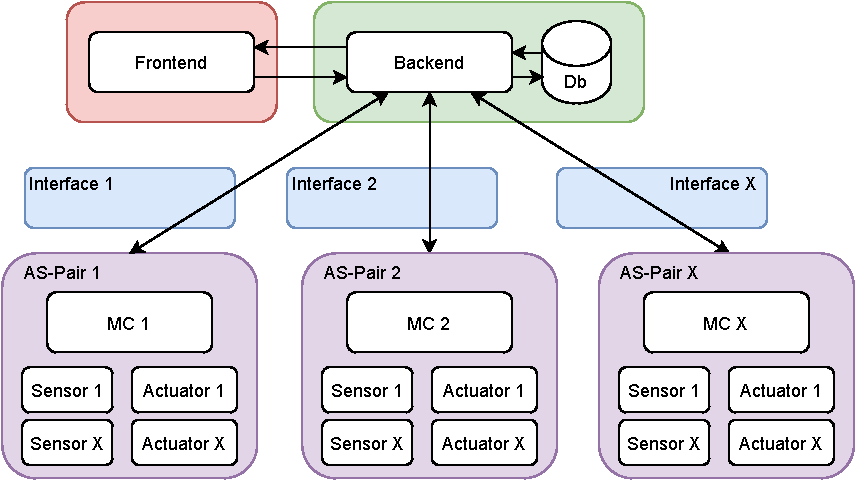
\includegraphics[width=.9\textwidth]{images/4_1/second_concept.pdf}
    \caption{A more detailed schematic representation of the system}
    \label{fig:scale_conc_system}
\end{figure}

For this project, the presented architecture in figure \ref{fig:scale_conc_system} is sufficient. However, if numerous AS-Pairs are required or numerous frontend requests are received, the bottleneck of the system occurs at the backend. If these cases occur, the system would have to be extended with additional backends and additional databases. For this purpose, the system must be extended by load balancers that handle the frontend requests and the communication with the AS pairs and the system can be extended with a database cluster.\\

